\documentclass[10pt,twocolumn,letterpaper]{article}
\usepackage[review]{cvpr}
\usepackage{graphicx,amsmath,amssymb,booktabs,mathtools,microtype,placeins}
\definecolor{cvprblue}{rgb}{0.21,0.49,0.74}
\usepackage[pagebackref,breaklinks,colorlinks,allcolors=cvprblue]{hyperref}
\def\confName{CVPR}
\def\confYear{2027}
\newcommand{\mm}{\,\mathrm{mm}}
\newcommand{\pp}{\,\mathrm{pp}}
\newcommand{\hu}{\,\mathrm{HU}}
\newcommand{\clip}{[\,\cdot\,]_+}
\newcommand{\PaperAbstract}{An exterior vessel forecast can change where a chest CT candidate scorer finds a lesion. We isolate that effect using lesion and control crops with identical exteriors and a smooth rotation of the same fitted field. At a matched 10\% candidate false-positive rate (FPR), correct placement recovered \(+6.09\pp\) (95\% CI \([+4.38,+7.78]\)) more insertions within 3 mm on a fresh broad-texture LUNA16 holdout (12,240 insertions, 170 patients). It recovered \(+2.76\pp\) (95\% CI \([+1.77,+3.76]\)) on 72 independent HiPaS release scans with annotated native vessels and inserted lesions. In the original low-texture study, alignment improved crop sensitivity by \(+9.37\pp\) (95\% CI \([+4.56,+12.29]\)). With the affine background, compact templates, search, and head matched, fixed subtraction localized more insertions than joint profiling on the broader holdout. The paired crop-sensitivity difference between those readouts spanned zero. These experiments identify forecast placement as a source of useful localization at a fixed candidate false-alarm budget.}
\newcommand{\IntroEvidence}{In the fresh LUNA16 holdout, a refitted rotated profile localized 7.35\% of the insertions at the 10\% candidate FPR cap. Correct placement raised that to 13.45\%. Alignment also improved the same endpoint on native vessel neighborhoods from an independent acquisition. In the original lower-texture condition the effect reached the crop decision itself. The two endpoints distinguish finding a better location from accepting more crops.}
\newcommand{\BroadResults}{The fresh holdout comprises 170 patients, 680 controls, and 12,240 insertions. The median unmodified core SD is \(117\hu\). At matched FPR, the sealed aligned profile raised crop sensitivity by \(+2.08\pp\) (95\% CI \([-0.27,+4.40]\)) over the refitted rotation and by \(+4.05\pp\) (95\% CI \([+1.37,+6.23]\)) over the rotation evaluated with the aligned head fixed. Its gain in localized acceptance over the refitted rotation was \(+6.09\pp\) (95\% CI \([+4.38,+7.78]\)) (Fig.~\ref{fig:localization}). Among crops that both arms accepted, alignment moved 386 from an off-target to an on-target peak and moved 124 the other way. Another 647 were localized after a rejection by the rotated arm, compared with 163 lost in the reverse direction. These transitions show how a change in the marked location can exceed the change in crop acceptance. At frozen cutoffs the sensitivity difference was \(+4.50\pp\), at achieved FPR 10.59\% versus 8.82\%. The joint calibration and test interval for the sensitivity difference was \([-0.59,+8.31]\pp\), and the paired excess-FPR upper limit was \(5.00\pp\). The prespecified broader crop criterion was unmet.}
\newcommand{\FocusedResults}{In the original locked experiment, alignment gained \(+9.66\pp\) (95\% CI \([+8.10,+11.19]\)) over rotation at 10.38\% versus 10.02\% achieved FPR. The gain at matched 10\% FPR was \(+9.37\pp\) (95\% CI \([+4.56,+12.29]\)). In the retrospective shared-readout comparison on those same cases, the fixed residual gained \(+14.72\pp\) (95\% CI \([+11.11,+17.05]\)) over its rotation and \(+14.15\pp\) (95\% CI \([+10.73,+16.44]\)) over shell summaries. The fixed readout gained 2,001 and lost 546 positive decisions relative to its rotation at the matched cap.}
\newcommand{\ReadoutResults}{The original profile-minus-Hessian difference was \(-0.84\pp\) (95\% CI \([-6.15,+2.43]\)) at the matched cap. On those viewed cases, replacing the Hessian with the matched fixed-residual head changed sensitivity by \(+3.41\pp\) (95\% CI \([-0.23,+6.05]\)). In the fresh broader holdout the profile difference relative to the strongest residual, fixed subtraction, was \(-0.74\pp\) (95\% CI \([-3.04,+0.54]\)). Fixed subtraction localized 15.38\% of all insertions and gained \(+1.93\pp\) (95\% CI \([+1.05,+3.27]\)) over profiling for that endpoint. With exact fields on 18 development backgrounds, fixed subtraction correctly ordered 67.6\% of the insertion/control pairs, compared with 62.0\% for plug-in and 67.6\% for profiling.}
\newcommand{\LearnedResults}{On development, the observed-CT CNN reached 67.54\% AUROC and 36.28\% sensitivity at the empirical FPR cap. The local ridge reached 68.08\% and 36.47\%, respectively. On the viewed focused test, the CNN placement difference was \(-0.54\pp\) (95\% CI \([-2.80,+0.62]\)). Its residual-channel arm changed sensitivity by \(+2.16\pp\) (95\% CI \([-1.19,+4.44]\)) over the observed-CT CNN. The learned comparison supports a useful local classifier, with intervals spanning zero for the effect of the additional spatial channel.}
\newcommand{\ConditionResults}{At the broader study's global FPR cap, the matched crop-sensitivity gain was \(+15.40\pp\) (95\% CI \([+11.84,+19.08]\)) for the strongest displaced insertions. The corresponding changes were \(-5.34\pp\) (95\% CI \([-9.49,-1.25]\)) for centered insertions, \(-1.47\pp\) (95\% CI \([-2.60,-0.24]\)) for the faintest contrast, and \(-0.12\pp\) (95\% CI \([-3.59,+3.23]\)) for at least 50\% overlap. The focused fixed-residual comparison also concentrated gains on the stronger displaced cases (Fig.~\ref{fig:strata}).}
\newcommand{\DominanceResults}{The high-dominance band covered 40.7\% of broader crops. Its sensitivity difference was \(+3.29\pp\) (95\% CI \([+0.04,+6.03]\)). The high-minus-low interaction was \(+2.03\pp\) (95\% CI \([-1.62,+5.11]\)). The remaining band contained 7,254 insertions, with 5,631 misses by the aligned arm at the global matched threshold.}
\newcommand{\TransferResults}{On 72 fresh HiPaS scans, 7,713 of 7,776 inserted targets fell within 2 mm of a manual artery or vein label. At the matched candidate budget, alignment improved localized acceptance by \(+2.76\pp\) (95\% CI \([+1.77,+3.76]\)) and crop sensitivity by \(+1.36\pp\) (95\% CI \([-0.26,+3.69]\)) over the refitted rotation. The LUNA16 cutoffs yielded 2.15\% sensitivity at 0.69\% no-insertion acceptance for the aligned profile, versus 6.62\% at 4.63\% for its rotation.}
\newcommand{\CostResults}{At 65.0\% development coverage, bilateral selection reached 48.9\% sensitivity, compared with 47.9\% for forecast strength and 52.1\% for always using the aligned fixed residual. The bilateral policy took 137 ms per loaded crop on a single CPU thread, including its witness and selected readout. The strength policy took 132 ms and the always-aligned fixed residual took 133 ms.}
\newcommand{\PaperConclusion}{The paired CT intervention shows when exterior vascular evidence changes a candidate decision. Correct placement can release a competing maximum and return an inserted target at the same false-alarm budget. That localization effect persists when manually annotated native vessels replace artificial tubes. A fixed residual with a compact-template readout can exploit the same correspondence, making it a strong baseline for any more elaborate use of forecast uncertainty.}

\title{Beyond the Blob\\Localizing Inserted Lesions with Aligned Vessel Forecasts}
\author{}
\hypersetup{pdfauthor={},pdftitle={Beyond the Blob}}
\begin{document}
\raggedbottom
\maketitle

\begin{abstract}
\PaperAbstract{}
\end{abstract}

\section{Introduction}
A pulmonary vessel can present a compact cross-section, bend, or junction in a chest CT crop. A candidate classifier must decide whether a compact response is evidence of a lesion, while a local search must decide which response in the neighborhood deserves inspection. Even a credible model of the surrounding vessels can help or hurt these decisions. A forecast can explain away a competing vascular maximum, leave the maximum in place, or reduce the signal at the actual lesion. The effect depends on how the forecast lines up with the observed anatomy and on what the classifier does with the remaining signal.

We isolate the role of alignment using paired additions to CT crops. Each control and its corresponding lesion insertion share the same exterior, down to the voxel. The exterior supplies a forecast of the tubular structures that could cross the candidate. We then change where this same forecast is placed. An axial quarter-turn keeps its values, physical scales, and smoothness while breaking correspondence with the observed anatomy. A shell-summary control preserves aggregate evidence about the exterior. Both controls see the same candidate images. They allow a thresholded decision to be attributed to the placement of the forecast, beyond what can be achieved with a richer context vector.

\IntroEvidence{}

Two questions govern how to use this signal. The first is whether the same observation is scored better with a matched continuation than with a misplaced one. The second is whether a more flexible model of vessel amplitude improves on simply subtracting the exterior estimate. We hold the affine background, physical windows, compact templates, scale and location search, normalization, and fitted head family fixed across this comparison. Holding the vessel amplitude fixed, estimating it under the no-lesion hypothesis, and estimating it under both hypotheses give three different uses of the same evidence. A Hessian residual and a trained compact CNN provide complementary readouts.

Our contributions are a controlled test of spatial correspondence at a fixed candidate false-positive budget, a shared-readout comparison that isolates how much flexibility to give a vessel estimate, and a localization analysis that asks which compact response is recovered. We test with patient-disjoint calibration and newly rendered CT pairs, and use manually annotated native vessels in a separate transfer condition. Together these experiments identify a setting in which an aligned forecast changes what can be detected and where to look.

\begin{figure*}[t]
\centering
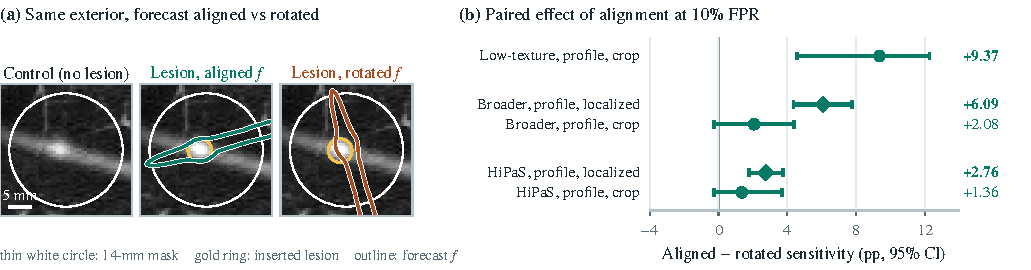
\includegraphics[width=\textwidth]{figures/placement.pdf}
\caption{\textbf{The same vessel forecast changes a decision when it is placed correctly.}
The axial development example shows the unmodified control and the inserted lesion, with the aligned and rotated forecast contours over the same lesion-present crop. The dashed ring delimits the masked region and the cross marks the center of the inserted footprint on this slice. All CT panels use the same display window. The paired differences on the right compare aligned and smooth-rotation arms at the empirical 10\% candidate FPR cap. Bars are 95\% intervals with shared patient blocks. The upper comparison uses the original locked low-texture study. The lower comparisons use the prespecified localization endpoint in the broad holdout and the native-vessel transfer.}
\label{fig:placement}
\end{figure*}

\section{Related work}
\paragraph{Vessels as explanations for compact responses.}
Multiscale Hessian filters describe local curvature and provide descriptors for tubular and compact structures \cite{frangi1998,sato1998,li2003}. They are natural components of candidate scoring. A junction can generate curvature along multiple axes, and the strongest response in a search region can lie away from the lesion. Agam \etal{} used reconstructed vessel trees to resolve local ambiguities in CT \cite{agam2005}. Charbonnier \etal{} used vessels outside supplied subsolid nodule contours to guide vessel segmentation within them \cite{charbonnier2018}. Learned candidate systems have also used local anatomy or multiple views \cite{wu2010,setio2016}. Gu \etal{} incorporated a vessel suppression branch in a nodule CAD system \cite{gu2020}. These approaches motivate the use of context. Our comparison fixes the exterior signal and changes its spatial correspondence with the candidate. It tests what the placement of a forecast contributes after matching the score construction and allowing the sham to be refitted.

\paragraph{Task-based assessment of image operations.}
A familiar concern in imaging is that a change in pixel fidelity can have a different effect on detectability. Li \etal{} compared denoising across detection observers, and Yu \etal{} found that image quality measures and detection efficiency can move in different directions \cite{li2021denoise,yu2023denoise}. Here the operation of interest is vascular subtraction or conditioning at a fixed crop. We examine performance after rectification, local normalization, and a spatial maximum. We use the same false-positive budget to compare scores, and ask whether the response sent for review is actually at the inserted target. The paired intervention also permits an exact-field check on a small set where the additive nuisance is known.

\paragraph{Detection with structured nuisance.}
Testing for a nonnegative signal in the presence of a structured interference subspace is a classical problem \cite{scharf1994}. We use a locally weighted affine model and a single exterior-derived nuisance column with an amplitude anchor. The comparison concerns the source and placement of the nuisance column, the treatment of amplitude uncertainty, and the effect on a searched candidate score. The stabilization floor, template search, and fitted classifier make the operating point an empirical property of the complete procedure.

\section{A controlled test of correspondence}
\label{sec:design}
\paragraph{The candidate decision.}
Each input is a fixed physical crop. A positive decision means that the crop is passed on for inspection. A second decision returns one coordinate inside the crop, where the readout places its strongest compact response. Figure~\ref{fig:workflow} separates the inputs to the exterior forecast from the inputs to the candidate scorer. The two decisions serve different purposes. A method can accept a lesion-bearing crop because a neighboring structure scored highly, and can improve the returned location on a crop that was already accepted. We measure both effects using known insertion coordinates.

\paragraph{Changing the observed target while holding context fixed.}
Let \(b\) be a CT background, \(v\) the added tubular field when used, and \(s\) an inserted lesion. The two images are \(y_0=b+v\) and \(y_1=b+v+s\), in linear intensity units. When using native vascular neighborhoods, \(v=0\) and the vessels are already part of \(b\). We require \(s=0\) throughout the visible exterior. The forecast \(f=F(y|_{\rm exterior})\) is therefore shared by a control and all of its insertions. All arms receive \(y_0\) and \(y_1\) at the same proposal center. The subtraction and profiling arms can use the complete observed crop. Only the forecasting step is masked.

This construction fixes the candidate population and removes an ambiguity that arises when scores are compared on different proposals. A method can score more highly because a lesion is present, and the observation carrying the lesion may affect a fitted amplitude inside the crop. It cannot change the forecast by changing a shell voxel. The controlled difference gives an intervention with a defined positive target, even at locations where the unmodified background contains complex anatomical structure.

\paragraph{Changing placement while holding the forecast fixed.}
We apply a 90-degree turn about the slice axis through the proposal center. The row and column spacings are equal, so the operation is a permutation without interpolation on the scored support. It preserves radial support and the voxel value multiset. It also preserves the spatial smoothness and the shape of the forecast. At nonzero radii its values generally move to different locations. Any forecast whose symmetry makes it invariant to the turn remains a valid case in the denominator. We compare the aligned field with a separately refitted rotated arm and with the aligned head evaluated on rotated features. Refitting lets the control make the best use of a misplaced yet informative field. Fixing the head removes the effect of refitting. The nonspatial control receives shell and forecast summaries without location-specific features.

\begin{figure*}[t]
\centering
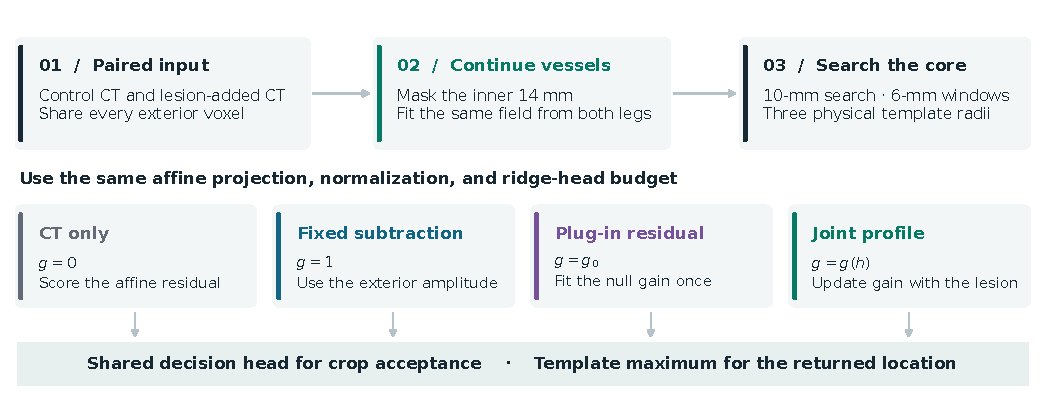
\includegraphics[width=\textwidth]{figures/workflow.pdf}
\caption{\textbf{One exterior, one physical search, four uses of the observation.}
The exterior beyond 14 mm supplies the fitted vessel field \(f\), shared by the control and every insertion on that background. For each location in the 10-mm core, the scorer uses a 6-mm weighted window and the same three compact templates. The local, fixed, plug-in, and profile arms differ in the vessel amplitude treatment. The same head family turns scale-specific maxima and shared features into a decision. The strongest template location supplies the localization endpoint.}
\label{fig:workflow}
\end{figure*}

\section{Readouts on a shared window bank}
\label{sec:method}
\paragraph{Forecasting from two visible legs.}
We represent each crop by \(64^3\) voxels at \(1.5\times0.7\times0.7\mm\) spacing in slice, row, and column coordinates. We mask everything within 14 mm for the forecast. Peaks on the 15.5-mm shell seed possible pairs of endpoints. We check for continuing signal against transverse flanks on both sides of each pair, at radii of 17.8 and 20.4 mm. For each accepted chord we fit a Gaussian cross-section and gain on the two exterior legs. Width and amplitude interpolate along the chord, with a smooth outer taper. This gives a real-valued additive estimate in CT units. A straight chord is a useful approximation when both legs support a continuation. Curved paths, branches, and other bright structures can produce disagreement. A crop with no accepted track has a zero forecast and is scored by the same procedure.

\paragraph{Affine residuals in physical windows.}
For each search center \(x\) within 10 mm of the proposal, take a 6-mm window and apply weights \(W_x\) with a Gaussian falloff of 3.4 mm. Let \(B\) span a constant and the three physical coordinates within this window. Project the observation, forecast, and compact template onto the \(W_x\)-orthogonal complement of \(B\), obtaining \(z,u,t\). The templates are
\[
T_{x,r}(p)=\bigl[1-\|p-x\|^2/r^2\bigr]_+^{0.8},
\qquad r\in\{1.85,2.7,3.7\}\mm .
\]
The affine projection removes background level and first-order drift. The amplitudes of \(z\), \(u\), and \(t\) are interpreted in the same weighted inner product. We fit a nonnegative template coefficient \(h\) to make the score directional in CT intensity.

\paragraph{The null and the choice of gain.}
With a vessel forecast, the null objective in one window is
\begin{equation}
J_0=\min_g \|z-gu\|_W^2+\lambda(g-1)^2,
\qquad \lambda=\rho\|u\|_W^2 .
\label{eq:null}
\end{equation}
For \(G=\|u\|_W^2+\lambda>0\), the fitted null gain is \(g_0=(\langle u,z\rangle_W+\lambda)/G\). A fixed residual uses \(g=1\) from the exterior fit. A plug-in residual uses \(g_0\) and holds it fixed when adding the compact template. A profiled score minimizes the penalized objective over \(g\) and \(h\geq0\) under the alternative. In the CT-only arm we set \(u=0\) and use the affine residual of \(y\). For an empty forecast all three vessel treatments reduce to the same local test before applying the fitted head.

For the plug-in arm the projection of the residual onto \(t\) is \(a=\langle t,z\rangle_W-g_0\langle t,u\rangle_W\). Adding a positive template reduces the loss by \([a]_+^2/d\), with \(d=\|t\|_W^2\). In the profile arm, the optimum vessel gain at any proposed \(h\) is \(g_0-h\langle t,u\rangle_W/G\). Eliminating it yields
\begin{equation}
J(h)=J_0-2ah+
  h^2\left(\|t\|_W^2-\frac{\langle t,u\rangle_W^2}{G}\right).
\label{eq:profile}
\end{equation}
The numerator is shared by plug-in and profile. Joint fitting changes the effective template norm. The two coincide where the forecast and template are orthogonal after affine projection. The profile score gives more relative weight to an otherwise identical positive residual correlation where the template and forecast overlap. In fixed subtraction, the numerator uses \(g=1\) and the null loss is the energy of that fixed residual. If an insertion lies where the fitted vessel is strong, a gain fitted from the observed core can absorb some of its signal. An amplitude fixed by the exterior protects against that change. Its tradeoff is sensitivity to amplitude error in the continuation.

The profiled objective can also be expressed using \(r=y-f\) and a correction \(\delta=g-1\). Retaining \(f\) makes this a change of coordinates. The arms differ by the treatment of the nuisance column and the chosen readout. A simple residual image can retain a useful lesion response even if a specific downstream statistic ranks the pair differently.

The null amplitude is especially important at a location where the lesion and vessel columns are correlated. Consider an observation \(z=z_0+h_\star t\) for a matched template at the insertion. At fixed \(u\) and \(G\), the fitted null gain changes by \(h_\star\langle u,t\rangle_W/G\). The plug-in residual correlation therefore increases by \(h_\star(\|t\|_W^2-\langle u,t\rangle_W^2/G)\), while the fixed residual correlation increases by \(h_\star\|t\|_W^2\). This comparison is local and holds before normalization. It shows why the same inserted signal can yield different increases even when the field is shared by the pair. Joint profiling compensates in the template norm and may also move the winning radius or center. On the other hand, keeping the gain fixed leaves any amplitude error in the exterior continuation in the residual. The measured decision gain depends on both effects and on competing locations elsewhere in the crop.

\paragraph{Common normalization and search.}
At each center and radius we take the nonnegative square root of the loss improvement and divide it by
\begin{equation}
\sigma_0=\sqrt{J_0/\sum W_x+\tau^2},
\end{equation}
using the null loss for that arm. We use the same normalization form and three floors in every arm. The profile template energy has a common positive numerical floor. We maximize over physical centers for each of the three template radii. Separately, the largest standardized template response across centers and radii gives the location sent for review. The reported crop decision also uses common observed-image features. The fitted ridge-logistic head receives 12 local intensity and Hessian summaries, three compact-template maxima from a larger affine projection, and three locally standardized CT-only maxima. The shell-only arm adds four exterior summaries. Each vessel-conditioned arm receives those same summaries and three additional vessel-conditioned maxima. Fixed, plug-in, and profile arms use identical feature counts and regularization budgets.

\paragraph{Comparator strength.}
The Hessian comparison subtracts the same exterior-fitted field before applying the conventional three-scale curvature statistic. Its three subtraction strengths include full subtraction. It therefore measures how much changing the readout can contribute when the nuisance estimate stays fixed. A separate hybrid CNN has a small learned 3D feature extractor and a shared observed-CT feature path. Its arms keep the same architecture, data, seeds, and optimization budget, and swap the second input between smoothed CT, aligned forecast, rotated forecast, and residual. This comparison asks whether the effect of placement carries over to a competitive learned scorer. The supplement reports its fitting checks and learning curves.

\section{Calibration and test protocol}
\label{sec:protocol}
\paragraph{Controlled source and shift.}
The focused LUNA16 experiment uses 549 proposal neighborhoods in 183 held-out patients, with 18 insertions per neighborhood. Each control has a single, crossing, or skew additive vessel configuration. The unmodified core SD is capped at \(42\hu\) to isolate cases in which those structures can compete strongly with the lesion. The original analysis froze its own fit, development and calibration roles, including 276 independent negative crops. We retain its original interpretation. We use the focused cases retrospectively to compare matched readouts and train and check the hybrid scorer on the original fit and development roles. Thus the new matched results on those 183 patients are development evidence.

The fresh LUNA16 experiment broadens the texture and morphology while retaining a shared additive nuisance. We sample four neighborhoods per patient in parenchymal CT, separated from published included and excluded findings and far enough from the scan boundary for the scorer \cite{setio2017,armato2011}. This cohort uses a new roster disjoint from the focused experiment and new spatial and insertion seeds. There is no ceiling on the unmodified core SD. Tubes can bend and taper. The lesion bank contains asymmetric bilobed and part-solid-like signals with independent orientation, three peak contrasts (84, 196, and \(364\hu\)), and offsets of 0, 4, and 7 mm relative to the proposal. These shapes differ from the radially decreasing search templates. Their support remains inside the mask. We reserve every eligible background in the locked test roster and use a separate patient pool for negative calibration.

The transfer condition uses a different noncontrast CT source, HiPaS, and its released manual artery and vein annotations \cite{chu2025hipas}. We sample neighborhoods between nearby annotated surfaces and insert the same morphology bank on untouched vascular backgrounds. These pairs separate the effect of removing artificial vessels from the effect of using the new lesion bank. A control is a crop with no added target. We use the annotations to measure distance and overlap and to set the sampling population. At inference the score uses the image alone. The transfer unit is the release scan.

\paragraph{Fit, select, calibrate.}
We fit the broader logistic heads on 80 background patients and select on another 85. Each arm has three settings. They couple the ridge-head regularization with the normalization floor and, when present, the gain penalty. We preselect the lead aligned arm, the strongest alternate residual, and the corresponding refitted rotation by sensitivity at the development 10\% candidate FPR cap. The study protocol freezes these identities, the cohort, the full insertion bank, and the analysis before rendering the reserved test images. We set a practical target of five additional accepted insertions per 100 at the same candidate false-alarm cap, with a positive paired lower confidence limit against both the rotation and the strongest residual. A development block-bootstrap calculation informs the sample size. The supplement gives the assumptions and the separate criteria for a transferred operating point.

At deployment-style cutoffs, each arm scores the same \(700\) negative crops from \(175\) independent LUNA16 calibration patients. We accept scores strictly above the order statistic that limits the calibration acceptance rate to 10\%. Ties at the cutoff are rejected. We apply these cutoffs unchanged to the broader holdout and the HiPaS transfer. The realized candidate FPR can differ among arms. A sensitivity difference at these cutoffs must be read together with its achieved FPR.

\paragraph{Estimands and uncertainty.}
The empirical ROC comparison sets each arm to the same 10\% candidate FPR cap within the evaluation cohort. A sample order statistic implements that cap. This comparison describes ranking at the target budget. The frozen analysis describes what happens when the threshold comes from independent calibration. We report both because they answer different operational questions. For localization, the crop must pass the same threshold and the returned peak must be within 3 mm of the known insertion center. Candidate FPR still counts all accepted controls. A localizer gains credit for changing the returned location on an already accepted crop.

We resample 3,000 shared patient blocks, stratified by release fold, keeping the entire insertion grid and all control crops for each draw. HiPaS is resampled by scan. For ROC intervals the test negative rank is recomputed inside every draw. For fixed thresholds we report conditional intervals and separately draw calibration blocks independently of the test blocks. This second calculation measures how threshold uncertainty changes sensitivity and false-positive comparisons across repetitions of the procedure. We use absolute percentage-point differences throughout.

\section{What correct placement buys}
\label{sec:results}
\BroadResults{}

\begin{table*}[t]
\centering
\small
\begin{tabular}{@{}lrrrrr@{}}
\toprule
& Focused, viewed & \multicolumn{4}{c}{Broader LUNA16, fresh holdout} \\
\cmidrule(lr){3-6}
Readout & Matched sens. & Matched sens. & Localized sens. & Frozen sens. & Frozen FPR \\
\midrule
Observed CT only & 32.88 & 21.39 & 13.37 & 23.78 & 11.62 \\
CT + shell summaries & 36.60 & 21.50 & 13.49 & 21.66 & 10.29 \\
Hessian subtraction & 47.34 & 14.31 & -- & 14.31 & 10.29 \\
Fixed subtraction, aligned & 50.75 & 24.05 & 15.38 & 24.74 & 10.59 \\
Fixed subtraction, rotated & 36.03 & 20.81 & 5.72 & 21.18 & 10.15 \\
Plug-in residual, aligned & 39.45 & 22.54 & 11.54 & 23.86 & 10.44 \\
Plug-in residual, rotated & 37.39 & 21.26 & 6.92 & 19.81 & 9.12 \\
\textbf{Joint profile, aligned} & \textbf{46.50} & \textbf{23.32} & \textbf{13.45} & \textbf{23.79} & \textbf{10.59} \\
Joint profile, rotated & 37.13 & 21.23 & 7.35 & 19.29 & 8.82 \\
Profile, rotated with fixed head & -- & 19.26 & 9.19 & 19.20 & 10.00 \\
\midrule
Lead $-$ refitted rotation & -- & +2.1 [-0.3, +4.4] & +6.1 [+4.4, +7.8] & -- & -- \\
Lead $-$ strongest residual & -- & -0.7 [-3.0, +0.5] & -1.9 [-3.3, -1.0] & -- & -- \\
\bottomrule
\end{tabular}

\caption{\textbf{Matched placement and amplitude comparisons.}
The left column of results reuses the focused study for development. The fresh broader holdout compares the same families with separate fits and settings selected on broad development. The matched column uses the empirical 10\% candidate FPR cap. The frozen columns report the sensitivity and achieved candidate FPR together, in percent. Localization requires acceptance and a peak within 3 mm. Bold identifies the lead selected before testing. The contrast rows give paired 95\% intervals in percentage points.}
\label{tab:decisive}
\end{table*}

\paragraph{The placement effect in the focused experiment.}
\FocusedResults{}
The rotated and shell-only comparisons answer different questions. A rotation asks whether a field of comparable shape and strength helps as much after its anatomical correspondence is removed. Shell summaries ask whether aggregate context can account for the same decision gain. The aligned arm can use both sources of evidence. The paired gains beyond these controls isolate what the forecast supplies through its location.

\paragraph{How much amplitude flexibility is needed?}
\ReadoutResults{}
The fixed and profiled scores can both exploit correspondence. Their behavior reflects how the detector values a residual at the lesion location and how it handles overlapping nuisance and lesion directions. In the compact exact-field diagnostic, the forecast equals the added nuisance. Allowing the null gain to vary then changes the residual using the observation that may contain a lesion. The diagnostic is small and uses known additive truth. It helps interpret the matched score differences, while the thresholded comparison on the whole cohort determines which behavior is useful.

\begin{figure*}[t]
\centering
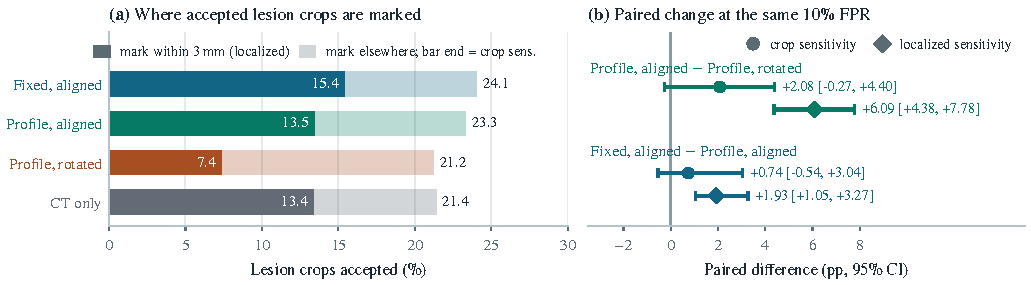
\includegraphics[width=\textwidth]{figures/localization.pdf}
\caption{\textbf{Acceptance and localization are separate decisions.}
Left, accepted positive crops on the broader holdout at the matched 10\% FPR cap, partitioned into peaks within 3 mm of the insertion and peaks farther away. The plotted methods use the same physical search and the same set of positive crops. Right, paired differences in ordinary and localized sensitivity, with 95\% patient-block intervals. Both decisions charge the same false-positive budget.}
\label{fig:localization}
\end{figure*}

\paragraph{A competent learned comparison.}
\LearnedResults{}
The hybrid scorer can combine spatial channels with the shared CT statistics. The result shows why the placement gain should be attached to the measured readout. A field can give a structured detector an explicit way to remove a rival response, while another classifier using the same crop and field may pool features that only weakly depend on their correspondence.

\section{Where alignment helps}
\label{sec:conditions}
\paragraph{What the localization endpoint adds.}
Write \(A(y)\) for the crop acceptance event, \(L(y)\) for the reported location, and \(Y=1\) for an insertion at center \(x_\star\). At a given false-positive cap, localized sensitivity is
\[
\Pr\bigl(A(y)=1,\ \|L(y)-x_\star\|\leq 3\mm\mid Y=1\bigr).
\]
It depends on the accepted set and on where the template map peaks within that set. To see how placement can change one without the other, consider two competing template responses \(m(x_\ell)\) and \(m(x_v)\) near the lesion and a vessel. Suppose the vessel leads before conditioning. If conditioning reduces the two responses by \(d_\ell\) and \(d_v\), the lesion overtakes the vessel when \(d_v-d_\ell > m(x_v)-m(x_\ell)\), provided the remaining locations score lower. The crop classifier can accept both crops even while this ordering changes. The expression applies to the standardized response and allows either signed change. It avoids treating subtraction as a constant shift of the full response map.

This distinction is visible in the paired transitions. Among the broader crops that switch to a correctly localized mark under alignment, a substantial group already passed the rotated score. On HiPaS, both types of change occur as well. In these cases the gain is in the location a reviewer would see. At the same time, some previously correct marks move off target. We count those losses, keep control acceptances in the denominator, and use each arm's global cutoff across conditions. The supplement reports the transition counts and a cross-check with the fixed residual.

\paragraph{Competition inside the search region.}
\ConditionResults{}
An off-center insertion can be missed when the proposal is anchored on a different bright response. A helpful continuation puts its nuisance explanation at that competing response, leaving the template search free to return the target. A centered lesion can already coincide with the most conspicuous response. A faint lesion offers a weak residual even when the competing vessel is explained well. The conditional analyses separate these situations at the global candidate thresholds. True offsets and overlap describe the controlled cases and are used for analysis after scoring.

\begin{figure*}[t]
\centering
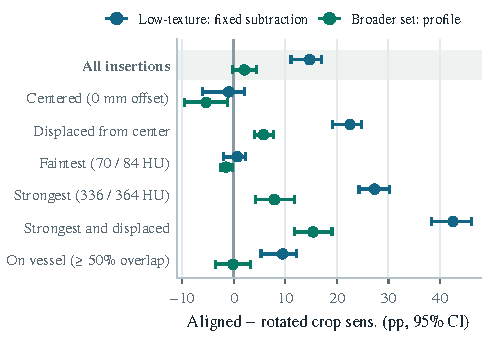
\includegraphics[width=\textwidth]{figures/strata.pdf}
\caption{\textbf{Placement gains by insertion condition at the global operating budget.}
Differences in sensitivity between aligned and refitted rotated arms at each study's overall empirical 10\% FPR cap. The focused columns show the development-selected fixed residual on viewed cases. The broader columns show the sealed lead on fresh cases. Stratum definitions and sizes follow the respective insertion banks. Bars are paired 95\% patient-block intervals. These are conditional diagnostics on the scored populations.}
\label{fig:strata}
\end{figure*}

\paragraph{A scoreable measure of forecast dominance.}
We also measure whether exterior continuation has high predicted amplitude relative to the residual contrast spread in the visible shell. The split is fixed at the broad development median. Its inputs are available to a candidate scorer before any test decision. \DominanceResults{}
This descriptive comparison uses one global threshold per method. It does not optimize a separate cutoff in the favorable band. The excluded-band misses and false-positive rates in the supplement make the coverage tradeoff explicit.

\paragraph{Native vessels and acquisition transfer.}
\TransferResults{}
Figure~\ref{fig:native} places the two transfer estimands side by side. The aligned fixed residual and profile occupy a similar range in localized sensitivity, and the local and shell arms show how much of this endpoint is available without spatial conditioning. Under the imported thresholds, several arms accept very few HiPaS controls. This downward shift in both acceptance and false alarms explains why the within-transfer ranking result and a transferred decision rule tell different stories. It also shows why independent negatives from the target acquisition would matter for a deployment-style claim.

The HiPaS transfer samples vessel-rich neighborhoods and uses an insertion control for each one. It tests whether the placement effect persists when real vascular anatomy supplies the competing background, including structures that a straight forecast fits imperfectly. A native nodule evaluation would need complete reference nodules and irrelevant findings and a verified patient and detector exposure audit. These paired insertions establish the controlled endpoints on the scored populations.

\begin{figure*}[t]
\centering
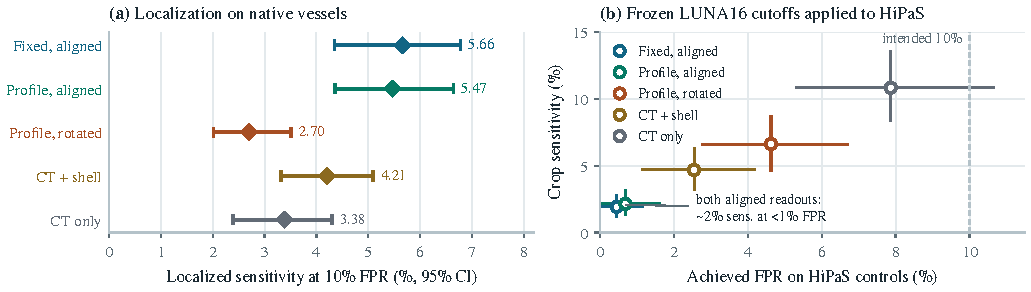
\includegraphics[width=\textwidth]{figures/native_transfer.pdf}
\caption{\textbf{Correct localization transfers to annotated native vessel backgrounds.}
Left, localized sensitivity for the 7,776 insertions on 72 HiPaS scans, at the within-transfer 10\% candidate FPR cap. Right, crop sensitivity and achieved FPR under the independent LUNA16 calibration cutoffs. Colors and symbols identify the same five readouts. Bars show 95\% scan-block intervals, conditional on the fixed cutoffs in the right panel.}
\label{fig:native}
\end{figure*}

\section{Discussion}
\label{sec:discussion}
\paragraph{What the comparison changes for a candidate scorer.}
Spatial evidence is valuable when its location is used in a way that can compete with a local maximum. The shape and amplitude of a forecast alone give it multiple routes to appear useful, including correlations with the type of background in the crop. The paired rotation, shell summary, and shared readout identify the additional contribution of correspondence. One implication is to compare a candidate method against a strength-preserving placement sham before attributing a gain to geometry. A second is to include the fixed residual with the same downstream search as an early benchmark. It uses the exterior estimate directly and exposes any benefit of a more flexible nuisance model.

The two endpoints offer a way to judge what kind of improvement matters. If a pipeline sends a marked location to a reviewer, relocating a response to the inserted lesion is consequential even when the total number of accepted crops changes little. Conversely, a gain in crop sensitivity can overstate what the mark shows when the peak falls on the original vessel. Localization in the controlled test supplies this check with a known target coordinate. Pairwise comparison on the same backgrounds also gives the gained and lost decisions. It exposes turnover that a difference of two mean sensitivities would hide.

\paragraph{Choosing when to use an intervention.}
The paired test diagnoses how geometry and readout change decisions. A per-candidate selection policy is a separate target. We tested one rule that falls back to a nonspatial score when the two exterior legs give weak agreement. It had the same development coverage options as a forecast-strength rule. \CostResults{}
The measured scope is candidate scoring from loaded CT. A prospective policy comparison would additionally require a sealed selector, full intervention costs, and paired quality at comparable total cost. Our scientific claim concerns the effect of forecast placement and amplitude treatment for specified readouts.

\paragraph{Interpreting operating points.}
The focused study's original primary criterion included an upper paired excess-FPR bound of 4 pp relative to the local head. Its observed upper limit was \(4.92\pp\). The two shifted conditions did not satisfy their full transfer criteria. These outcomes explain why a matched-FPR comparison and an independent calibration analysis belong together. A positive matched ROC effect establishes ranking separation at the specified budget. A shift in the negative score distribution can change the realized budget at an imported threshold. The fresh study's independent calibration bootstrap measures this part of the uncertainty directly. Differences in the source and prevalence of competing structures can still dominate nominal calibration precision.

\paragraph{Scope.}
The positive target in every new crop is an inserted signal. The broader LUNA16 experiment varies CT texture and morphology under a known intervention, and HiPaS adds an independently annotated native vascular background. Clinical nodules and scan-level proposal pipelines introduce further variation, including morphology, partial-volume effects, missed proposals, and differences in the denominator for false positives. A candidate rate on selected crops corresponds to this experiment's review budget. An independently adjudicated scan-level study would quantify clinical detection and false positives per scan.

\section{Conclusion}
\PaperConclusion{}

\FloatBarrier
\section*{LLM Usage Statement}
OpenAI Codex assisted with study design, implementation, experiment execution, numerical analysis, literature lookup, figure preparation, and manuscript drafting and editing. The quantitative figures were generated programmatically from recorded measurements. The qualitative panels use public CT crops or algorithmically specified phantoms. The authors are responsible for validating the work and its interpretation.

{\small
\bibliographystyle{ieeenat_fullname}
\bibliography{references}
}
\end{document}
